\documentclass[tikz,border=10pt]{standalone}
\usepackage[T1]{fontenc}
\usepackage{helvet}
\renewcommand{\familydefault}{\sfdefault}
\usepackage{amsmath,amssymb}
\usepackage{tikz}
\usetikzlibrary{calc,positioning,fit,arrows.meta,shapes.geometric}

% Canonical Academic Palette
\definecolor{OxfordNavy}{HTML}{1E293B}
\definecolor{SlateSteel}{HTML}{334155}
\definecolor{MutedTeal}{HTML}{0F766E}
\definecolor{TealL0}{HTML}{F0FDFA}
\definecolor{Burgundy}{HTML}{991B1B}
\definecolor{BurgundyL0}{HTML}{FEF2F2}
\definecolor{WarmOchre}{HTML}{92400E}
\definecolor{OchreL0}{HTML}{FFFBEB}
\definecolor{ForestSage}{HTML}{166534}
\definecolor{SageL0}{HTML}{F0FDF4}
\definecolor{CoolParchment}{HTML}{F8FAFC}
\definecolor{SlateRim}{HTML}{CBD5E1}
\definecolor{GoldPin}{HTML}{D97706}
\definecolor{DarkSlate}{HTML}{0F172A}
\definecolor{SiliconCarrier}{HTML}{1E222D}
\definecolor{InterposerTrace}{HTML}{0284C7}

\begin{document}
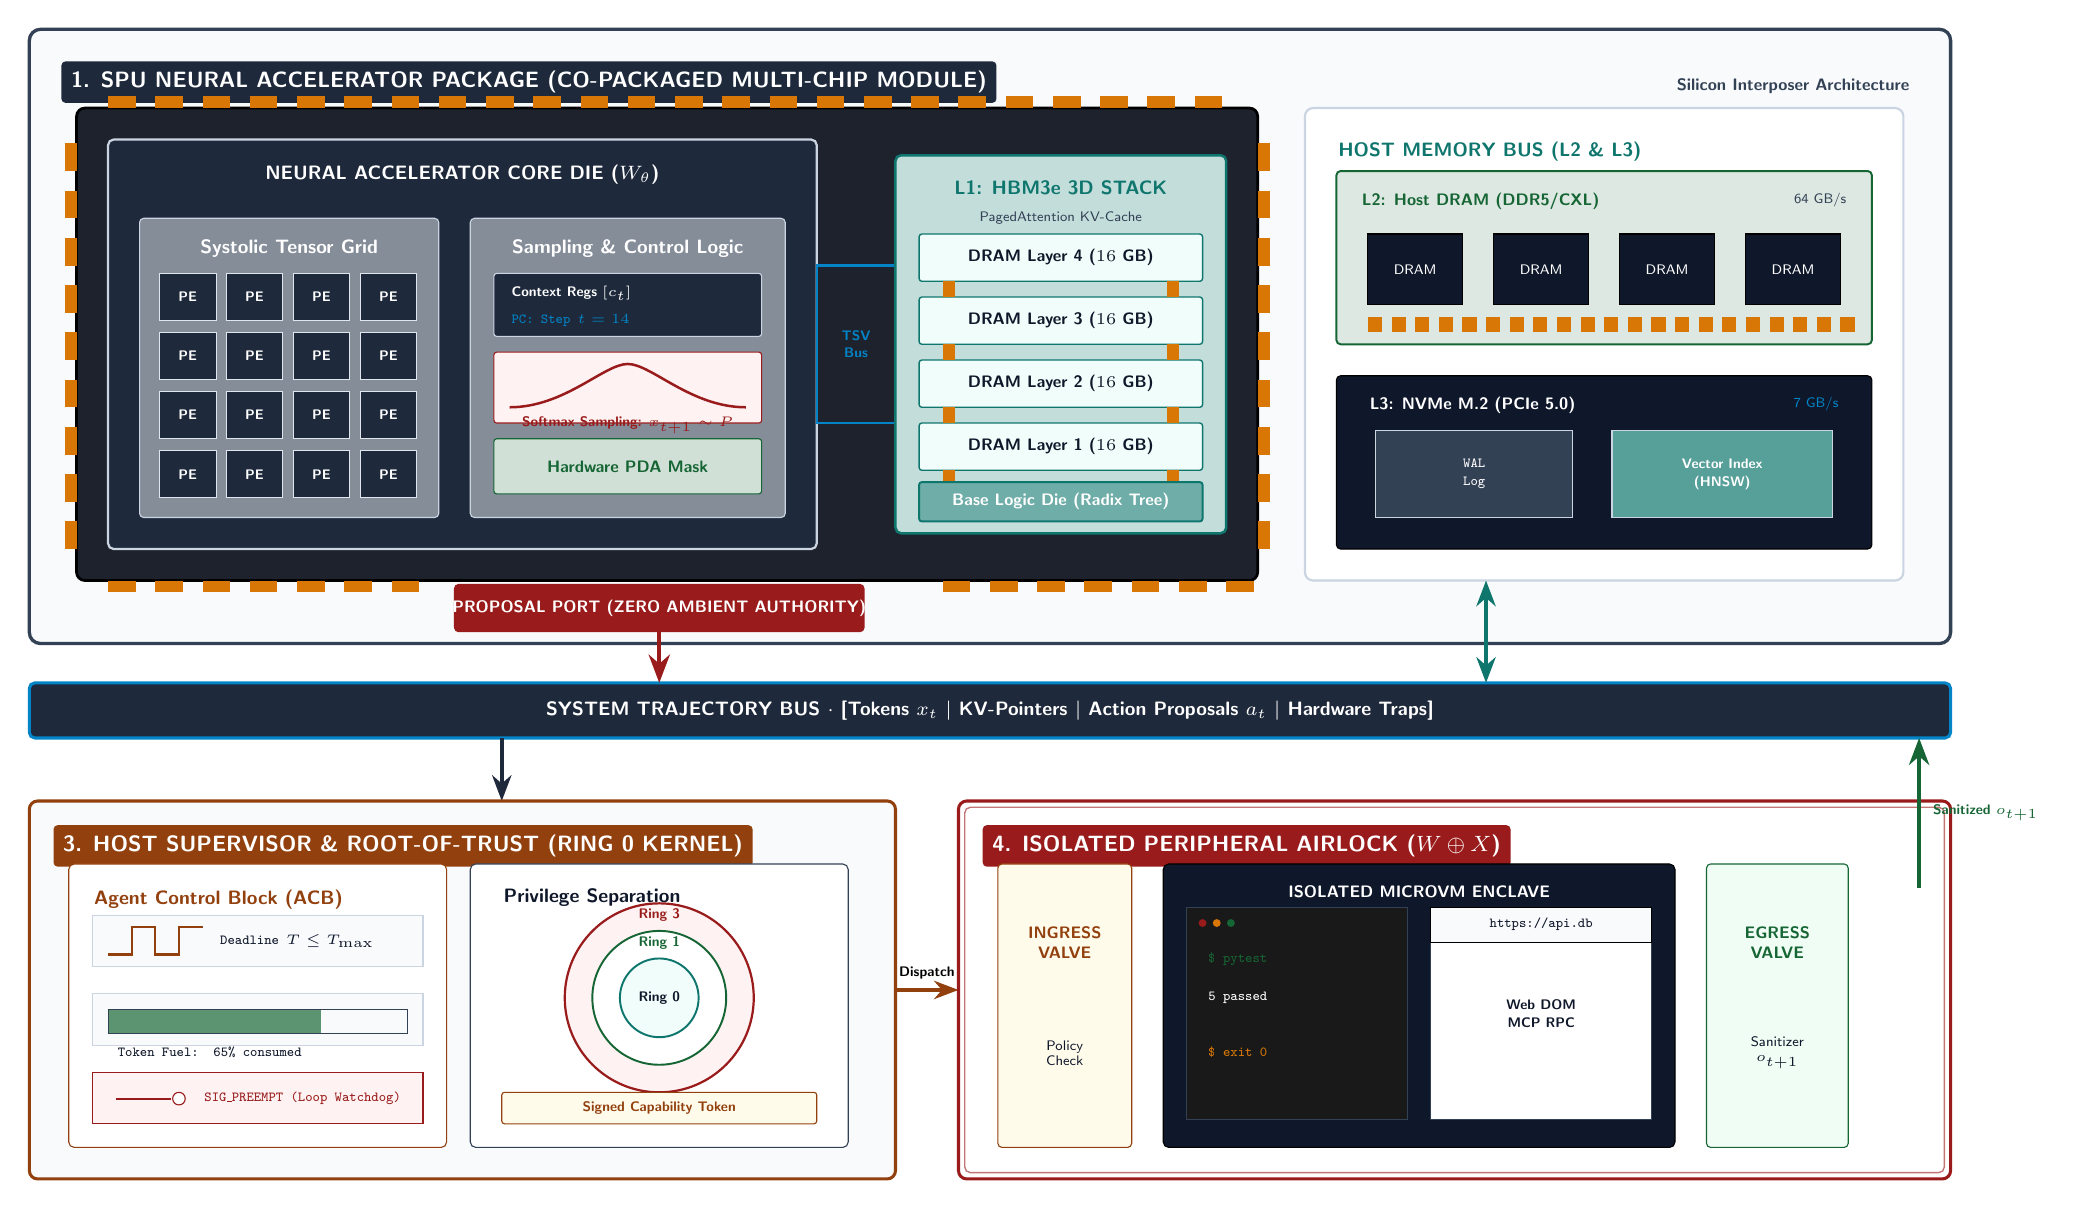
\begin{tikzpicture}[
  font=\sffamily,
  scale=1.0,
  >=Stealth
]

% -------------------------------------------------------------
% TOP HALF: CO-PACKAGED MULTI-CHIP MODULE (SPU + HBM ON INTERPOSER)
% -------------------------------------------------------------

% Physical Multi-Chip Carrier (Ceramic BGA Package)
\draw[fill=CoolParchment, draw=SlateSteel, line width=1.2pt, rounded corners=4pt]
  (0, 7.0) rectangle (24.4, 14.8);

\node[anchor=north west, fill=OxfordNavy, text=white, font=\fontsize{8.5}{10}\selectfont\bfseries, rounded corners=1.5pt, inner sep=3.5pt]
  at (0.4, 14.4) {1. SPU NEURAL ACCELERATOR PACKAGE (CO-PACKAGED MULTI-CHIP MODULE)};
\node[anchor=north east, text=SlateSteel, font=\fontsize{6.5}{8}\selectfont\bfseries]
  at (24.0, 14.3) {Silicon Interposer Architecture};

% Ceramic Substrate Body (Dark Slate)
\draw[fill=SiliconCarrier, draw=black, line width=1.0pt, rounded corners=3pt]
  (0.6, 7.8) rectangle (15.6, 13.8);

% Peripheral Gold BGA Micro-Pins (with pin cutout at bottom center for Proposal Port)
\foreach \x in {1.0, 1.6, ..., 15.2} {
  \fill[GoldPin] (\x, 13.8) rectangle (\x+0.35, 13.95);
}
\foreach \x in {1.0, 1.6, 2.2, 2.8, 3.4, 4.0, 4.6, 11.6, 12.2, 12.8, 13.4, 14.0, 14.6, 15.2} {
  \fill[GoldPin] (\x, 7.65) rectangle (\x+0.35, 7.8);
}
\foreach \y in {8.2, 8.8, ..., 13.4} {
  \fill[GoldPin] (0.45, \y) rectangle (0.6, \y+0.35);
  \fill[GoldPin] (15.6, \y) rectangle (15.75, \y+0.35);
}

% SPU Compute Die (Logic Die)
\draw[fill=OxfordNavy, draw=SlateRim, line width=0.8pt, rounded corners=2pt]
  (1.0, 8.2) rectangle (10.0, 13.4);
\node[anchor=north, text=white, font=\fontsize{7.5}{9}\selectfont\bfseries] at (5.5, 13.2) {NEURAL ACCELERATOR CORE DIE ($W_\theta$)};

% Inside Logic Die: Left Systolic Grid
\begin{scope}[shift={(1.4, 8.6)}]
  \draw[fill=SlateSteel!60, draw=SlateRim, rounded corners=1.5pt] (0, 0) rectangle (3.8, 3.8);
  \node[anchor=north, text=white, font=\fontsize{6.8}{8}\selectfont\bfseries] at (1.9, 3.65) {Systolic Tensor Grid};
  \foreach \r in {0, 1, 2, 3} {
    \foreach \c in {0, 1, 2, 3} {
      \draw[fill=OxfordNavy, draw=SlateRim!60, line width=0.3pt]
        (0.25 + \c*0.85, 0.25 + \r*0.75) rectangle (0.25 + \c*0.85 + 0.72, 0.25 + \r*0.75 + 0.6);
      \node[text=white, font=\fontsize{4.2}{5}\selectfont\bfseries] at (0.25 + \c*0.85 + 0.36, 0.25 + \r*0.75 + 0.3) {PE};
    }
  }
\end{scope}

% Inside Logic Die: Right Sampler & Registers
\begin{scope}[shift={(5.6, 8.6)}]
  \draw[fill=SlateSteel!60, draw=SlateRim, rounded corners=1.5pt] (0, 0) rectangle (4.0, 3.8);
  \node[anchor=north, text=white, font=\fontsize{6.8}{8}\selectfont\bfseries] at (2.0, 3.65) {Sampling \& Control Logic};

  % Context Registers
  \draw[fill=OxfordNavy, draw=SlateRim, rounded corners=1pt] (0.3, 2.3) rectangle (3.7, 3.1);
  \node[anchor=west, text=white, font=\fontsize{5.5}{6.5}\selectfont\bfseries] at (0.4, 2.85) {Context Regs $[c_t]$};
  \node[anchor=west, text=InterposerTrace, font=\fontsize{5.5}{6.5}\selectfont\ttfamily] at (0.4, 2.5) {PC: Step $t = 14$};

  % Softmax Sampler Curve
  \draw[fill=BurgundyL0, draw=Burgundy, rounded corners=1pt] (0.3, 1.2) rectangle (3.7, 2.1);
  \draw[draw=Burgundy, line width=0.9pt] 
    (0.5, 1.4) .. controls (1.2, 1.4) and (1.7, 1.95) .. (2.0, 1.95)
    .. controls (2.3, 1.95) and (2.8, 1.4) .. (3.5, 1.4);
  \node[anchor=north, text=Burgundy, font=\fontsize{5.2}{6}\selectfont\bfseries] at (2.0, 1.4) {Softmax Sampling: $x_{t+1} \sim P$};

  % PDA Mask
  \draw[fill=ForestSage!20, draw=ForestSage, rounded corners=1pt] (0.3, 0.3) rectangle (3.7, 1.0);
  \node[text=ForestSage, font=\fontsize{5.8}{7}\selectfont\bfseries] at (2.0, 0.65) {Hardware PDA Mask};
\end{scope}

% Silicon Interposer Trace Bridge
\draw[fill=SiliconCarrier, draw=InterposerTrace, line width=0.8pt] (10.0, 9.8) rectangle (11.0, 11.8);
\node[text=InterposerTrace, font=\fontsize{5.0}{6}\selectfont\bfseries, align=center] at (10.5, 10.8) {TSV\\Bus};

% Co-Packaged 3D HBM3e Die Stack
\begin{scope}[shift={(11.0, 8.4)}]
  \draw[fill=MutedTeal!25, draw=MutedTeal, line width=0.9pt, rounded corners=2pt] (0, 0) rectangle (4.2, 4.8);
  \node[anchor=north, text=MutedTeal, font=\fontsize{7.2}{8.5}\selectfont\bfseries] at (2.1, 4.6) {L1: HBM3e 3D STACK};
  \node[anchor=north, text=SlateSteel, font=\fontsize{5.5}{6.5}\selectfont] at (2.1, 4.2) {PagedAttention KV-Cache};

  % 4 DRAM layers
  \foreach \y [count=\idx] in {0.8, 1.6, 2.4, 3.2} {
    \draw[fill=TealL0, draw=MutedTeal, line width=0.5pt, rounded corners=1pt] (0.3, \y) rectangle (3.9, \y+0.6);
    \node[text=DarkSlate, font=\fontsize{5.8}{7}\selectfont\bfseries] at (2.1, \y+0.3) {DRAM Layer \idx \ ($16\text{ GB}$)};
    \fill[GoldPin] (0.6, \y-0.2) rectangle (0.75, \y);
    \fill[GoldPin] (3.45, \y-0.2) rectangle (3.6, \y);
  }
  % Base Logic Die
  \draw[fill=MutedTeal!60, draw=MutedTeal, line width=0.7pt, rounded corners=1pt] (0.3, 0.15) rectangle (3.9, 0.65);
  \node[text=white, font=\fontsize{5.8}{7}\selectfont\bfseries] at (2.1, 0.4) {Base Logic Die (Radix Tree)};
\end{scope}

% External Memory Subsystem on Motherboard (L2 & L3)
\begin{scope}[shift={(16.2, 7.8)}]
  \draw[fill=white, draw=SlateRim, line width=0.8pt, rounded corners=3pt] (0, 0) rectangle (7.6, 6.0);
  \node[anchor=north west, text=MutedTeal, font=\fontsize{7.5}{9}\selectfont\bfseries] at (0.3, 5.7) {HOST MEMORY BUS (L2 \& L3)};

  % DDR5 Module
  \begin{scope}[shift={(0.4, 3.0)}]
    \draw[fill=ForestSage!15, draw=ForestSage, line width=0.7pt, rounded corners=1.5pt] (0, 0) rectangle (6.8, 2.2);
    \node[anchor=north west, text=ForestSage, font=\fontsize{6.5}{7.5}\selectfont\bfseries] at (0.2, 2.05) {L2: Host DRAM (DDR5/CXL)};
    \node[anchor=north east, text=SlateSteel, font=\fontsize{5.2}{6}\selectfont] at (6.6, 2.05) {64 GB/s};
    \foreach \x in {0.4, 2.0, 3.6, 5.2} {
      \draw[fill=DarkSlate, draw=black] (\x, 0.5) rectangle (\x+1.2, 1.4);
      \node[text=white, font=\fontsize{5.0}{6}\selectfont] at (\x+0.6, 0.95) {DRAM};
    }
    \foreach \p in {0.4, 0.7, ..., 6.5} {
      \fill[GoldPin] (\p, 0.15) rectangle (\p+0.18, 0.35);
    }
  \end{scope}

  % NVMe M.2 Drive
  \begin{scope}[shift={(0.4, 0.4)}]
    \draw[fill=DarkSlate, draw=black, rounded corners=1.5pt] (0, 0) rectangle (6.8, 2.2);
    \node[anchor=north west, text=white, font=\fontsize{6.5}{7.5}\selectfont\bfseries] at (0.3, 2.05) {L3: NVMe M.2 (PCIe 5.0)};
    \node[anchor=north east, text=InterposerTrace, font=\fontsize{5.2}{6}\selectfont] at (6.5, 2.05) {7 GB/s};
    \draw[fill=SlateSteel, draw=SlateRim] (0.5, 0.4) rectangle (3.0, 1.5);
    \node[text=white, font=\fontsize{5.5}{6.5}\selectfont\ttfamily, align=center] at (1.75, 0.95) {WAL\\Log};
    \draw[fill=MutedTeal!70, draw=SlateRim] (3.5, 0.4) rectangle (6.3, 1.5);
    \node[text=white, font=\fontsize{5.5}{6.5}\selectfont\bfseries, align=center] at (4.9, 0.95) {Vector Index\\(HNSW)};
  \end{scope}
\end{scope}

% Proposal Socket cleanly seated in pin cutout at bottom of SPU package
\draw[fill=Burgundy, draw=Burgundy, rounded corners=1.5pt] (5.4, 7.15) rectangle (10.6, 7.75);
\node[text=white, font=\fontsize{6.2}{7.5}\selectfont\bfseries] at (8.0, 7.45) {PROPOSAL PORT (ZERO AMBIENT AUTHORITY)};


% -------------------------------------------------------------
% MIDDLE: MOTHERBOARD TRAJECTORY BUS
% -------------------------------------------------------------
\draw[fill=OxfordNavy, draw=InterposerTrace, line width=1.1pt, rounded corners=2pt]
  (0, 5.8) rectangle (24.4, 6.5);
\node[text=white, font=\fontsize{7.2}{8.5}\selectfont\bfseries] at (12.2, 6.15) {
  SYSTEM TRAJECTORY BUS $\cdot$ [Tokens $x_t$ $\mid$ KV-Pointers $\mid$ Action Proposals $a_t$ $\mid$ Hardware Traps]
};

% Motherboard PCB via traces
\draw[->, draw=Burgundy, line width=1.6pt] (8.0, 7.15) -- (8.0, 6.5);
\draw[<->, draw=MutedTeal, line width=1.4pt] (18.5, 7.8) -- (18.5, 6.5);
\draw[->, draw=OxfordNavy, line width=1.4pt] (6.0, 5.8) -- (6.0, 5.0);


% -------------------------------------------------------------
% BOTTOM HALF: HOST ROOT-OF-TRUST & ISOLATED AIRLOCK
% -------------------------------------------------------------

% Host Supervisor Kernel
\begin{scope}[shift={(0, 0.2)}]
  \draw[fill=CoolParchment, draw=WarmOchre, line width=1.1pt, rounded corners=3pt]
    (0, 0) rectangle (11.0, 4.8);
  \node[anchor=north west, fill=WarmOchre, text=white, font=\fontsize{8.5}{10}\selectfont\bfseries, rounded corners=1.5pt, inner sep=3.5pt]
    at (0.3, 4.5) {3. HOST SUPERVISOR \& ROOT-OF-TRUST (RING 0 KERNEL)};

  % ACB
  \begin{scope}[shift={(0.5, 0.4)}]
    \draw[fill=white, draw=WarmOchre, rounded corners=2pt] (0, 0) rectangle (4.8, 3.6);
    \node[anchor=north west, text=WarmOchre, font=\fontsize{7.0}{8.5}\selectfont\bfseries] at (0.2, 3.4) {Agent Control Block (ACB)};

    % Clock waveform
    \draw[fill=CoolParchment, draw=SlateRim] (0.3, 2.3) rectangle (4.5, 2.95);
    \draw[draw=WarmOchre, line width=0.8pt] 
      (0.5, 2.45) -- (0.8, 2.45) -- (0.8, 2.8) -- (1.1, 2.8) -- (1.1, 2.45) -- (1.4, 2.45) -- (1.4, 2.8) -- (1.7, 2.8);
    \node[anchor=west, text=DarkSlate, font=\fontsize{5.0}{6}\selectfont\ttfamily] at (1.8, 2.62) {Deadline $T \le T_{\max}$};

    % Fuel progress bar
    \draw[fill=CoolParchment, draw=SlateRim] (0.3, 1.3) rectangle (4.5, 1.95);
    \fill[ForestSage!70] (0.5, 1.45) rectangle (3.2, 1.75);
    \draw[draw=SlateSteel, line width=0.3pt] (0.5, 1.45) rectangle (4.3, 1.75);
    \node[anchor=north west, text=DarkSlate, font=\fontsize{4.8}{5.5}\selectfont\ttfamily] at (0.5, 1.4) {Token Fuel: 65\% consumed};

    % Watchdog
    \draw[fill=BurgundyL0, draw=Burgundy] (0.3, 0.3) rectangle (4.5, 0.95);
    \draw[draw=Burgundy, line width=0.8pt] (0.6, 0.62) -- (1.3, 0.62);
    \draw[draw=Burgundy, fill=white] (1.4, 0.62) circle (0.08);
    \node[anchor=west, text=Burgundy, font=\fontsize{5.0}{6}\selectfont\ttfamily\bfseries] at (1.6, 0.62) {SIG\_PREEMPT (Loop Watchdog)};
  \end{scope}

  % Privilege Rings
  \begin{scope}[shift={(5.6, 0.4)}]
    \draw[fill=white, draw=SlateSteel, rounded corners=2pt] (0, 0) rectangle (4.8, 3.6);
    \node[anchor=north west, text=DarkSlate, font=\fontsize{7.0}{8.5}\selectfont\bfseries] at (0.3, 3.4) {Privilege Separation};

    \begin{scope}[shift={(2.4, 1.9)}]
      \draw[draw=Burgundy, fill=BurgundyL0, line width=0.8pt] (0, 0) circle (1.2);
      \node[anchor=south, font=\fontsize{4.8}{5.5}\selectfont\bfseries, text=Burgundy] at (0, 0.85) {Ring 3};
      
      \draw[draw=ForestSage, fill=white, line width=0.7pt] (0, 0) circle (0.85);
      \node[anchor=south, font=\fontsize{4.8}{5.5}\selectfont\bfseries, text=ForestSage] at (0, 0.5) {Ring 1};

      \draw[draw=MutedTeal, fill=TealL0, line width=0.7pt] (0, 0) circle (0.5);
      \node[font=\fontsize{5.0}{6}\selectfont\bfseries, text=DarkSlate] at (0, 0) {Ring 0};
    \end{scope}

    \draw[fill=OchreL0, draw=WarmOchre, rounded corners=1pt] (0.4, 0.3) rectangle (4.4, 0.7);
    \node[font=\fontsize{5.5}{6.5}\selectfont\bfseries, text=WarmOchre] at (2.4, 0.5) {Signed Capability Token};
  \end{scope}
\end{scope}

% Dispatch Trace
\draw[->, draw=WarmOchre, line width=1.3pt] (11.0, 2.6) -- (11.8, 2.6)
  node[midway, above, font=\fontsize{5.5}{6.5}\selectfont\bfseries] {Dispatch};

% Isolated Airlock Peripheral
\begin{scope}[shift={(11.8, 0.2)}]
  \draw[fill=white, draw=Burgundy, line width=1.1pt, rounded corners=3pt] (0, 0) rectangle (12.6, 4.8);
  \draw[draw=Burgundy!60, line width=0.5pt, rounded corners=2pt] (0.08, 0.08) rectangle (12.52, 4.72);

  \node[anchor=north west, fill=Burgundy, text=white, font=\fontsize{8.5}{10}\selectfont\bfseries, rounded corners=1.5pt, inner sep=3.5pt]
    at (0.3, 4.5) {4. ISOLATED PERIPHERAL AIRLOCK ($W \oplus X$)};

  % Ingress
  \begin{scope}[shift={(0.5, 0.4)}]
    \draw[fill=OchreL0, draw=WarmOchre, rounded corners=1.5pt] (0, 0) rectangle (1.7, 3.6);
    \node[font=\fontsize{6.5}{7.5}\selectfont\bfseries, text=WarmOchre, align=center] at (0.85, 2.6) {INGRESS\\VALVE};
    \node[font=\fontsize{4.8}{5.5}\selectfont, text=DarkSlate, align=center] at (0.85, 1.2) {Policy\\Check};
  \end{scope}

  % MicroVM
  \begin{scope}[shift={(2.6, 0.4)}]
    \draw[fill=DarkSlate, draw=black, rounded corners=2pt] (0, 0) rectangle (6.5, 3.6);
    \node[anchor=north, font=\fontsize{6.2}{7.5}\selectfont\bfseries, text=white] at (3.25, 3.45) {ISOLATED MICROVM ENCLAVE};

    \begin{scope}[shift={(0.3, 0.35)}]
      \draw[fill=black!90, draw=SlateSteel] (0, 0) rectangle (2.8, 2.7);
      \fill[Burgundy] (0.2, 2.5) circle (0.05);
      \fill[GoldPin] (0.38, 2.5) circle (0.05);
      \fill[ForestSage] (0.56, 2.5) circle (0.05);
      \node[anchor=north west, font=\fontsize{4.2}{5}\selectfont\ttfamily, text=ForestSage] at (0.15, 2.25) {\$ pytest};
      \node[anchor=north west, font=\fontsize{4.0}{5}\selectfont\ttfamily, text=white!85] at (0.15, 1.75) {5 passed};
      \node[anchor=north west, font=\fontsize{4.2}{5}\selectfont\ttfamily, text=GoldPin] at (0.15, 1.05) {\$ exit 0};
    \end{scope}

    \begin{scope}[shift={(3.4, 0.35)}]
      \draw[fill=white, draw=SlateSteel] (0, 0) rectangle (2.8, 2.7);
      \draw[fill=CoolParchment] (0, 2.25) rectangle (2.8, 2.7);
      \node[font=\fontsize{4.0}{5}\selectfont\ttfamily, text=DarkSlate] at (1.4, 2.48) {https://api.db};
      \node[font=\fontsize{5.5}{6.5}\selectfont\bfseries, text=DarkSlate, align=center] at (1.4, 1.35) {Web DOM\\MCP RPC};
    \end{scope}
  \end{scope}

  % Egress
  \begin{scope}[shift={(9.5, 0.4)}]
    \draw[fill=SageL0, draw=ForestSage, rounded corners=1.5pt] (0, 0) rectangle (1.8, 3.6);
    \node[font=\fontsize{6.5}{7.5}\selectfont\bfseries, text=ForestSage, align=center] at (0.9, 2.6) {EGRESS\\VALVE};
    \node[font=\fontsize{4.8}{5.5}\selectfont, text=DarkSlate, align=center] at (0.9, 1.2) {Sanitizer\\$o_{t+1}$};
  \end{scope}
\end{scope}

% Feedback loop to Trajectory Bus
\draw[->, draw=ForestSage, line width=1.5pt] (24.0, 3.9) -- (24.0, 5.8)
  node[midway, right=1pt, font=\fontsize{5.5}{6.5}\selectfont\bfseries, text=ForestSage] {Sanitized $o_{t+1}$};

\end{tikzpicture}
\end{document}
